\documentclass{article}


% Packages
\usepackage{fullpage}
\usepackage{amssymb}
\usepackage{multicol}
\usepackage{amsmath}
\usepackage{amsfonts}
\usepackage{bm}
\usepackage{float}
\usepackage{tikz}
\usepackage{xcolor}
\usetikzlibrary{shapes.geometric, positioning, arrows, intersections}
\usepackage{amsthm}
\usepackage{hyperref}
\hypersetup{
    colorlinks=true, %set true if you want colored links
    linktoc=all,     %set to all if you want both sections and subsections linked
    linkcolor=black,  %choose some color if you want links to stand out
}

% Macros
\newcommand{\R}{\mathbb{R}}
\newcommand{\N}{\mathbb{N}}
\newcommand{\Q}{\mathbb{Q}}
\newcommand{\sub}{\subset}
\renewcommand{\a}{\alpha}
\renewcommand{\b}{\beta}
\newcommand{\g}{\gamma}
\renewcommand{\d}{\delta}
\newcommand{\e}{\varepsilon}
\newcommand{\ex}{\exists\,}
\newcommand{\overbar}[1]{\mkern 1.5mu\overline{\mkern-1.5mu#1\mkern-1.5mu}\mkern 1.5mu}
\newcommand{\eR}{\overbar{\R}}

\setlength{\columnsep}{20pt}

%ToC stuff
\newtheoremstyle{mythmstyle}%
    {}%
    {}%
    {\it}%
    {}%
    {\bf}%
    {}%
    { }%
    {\thmname{#1}\thmnumber{ #2}%
    \thmnote{: #3\addcontentsline{toc}{subsubsection}{{\it#1}: \tt#3}}. }
\theoremstyle{mythmstyle}
\newtheorem{theorem}{Theorem}[subsection]
\newtheorem{example}{Example}
\newtheorem{solution}{Solution}
\newtheorem{definition}{Definition}[subsection]
\newtheorem{corollary}{Corollary}

 % Document stuff

\title{Week 2: Limits and Functions}
\author{James Arthur}

\begin{document}
\maketitle
\tableofcontents
\newpage

\multicols{2}

\section{Limits}
\subsection{Defining Limits}

We consider limits of real functions, that is $f: X \to \R$, with $X\sub\R$.

\noindent\fbox{\parbox{0.475\textwidth}{\begin{definition}[Limit]{
 We say that $f(x)$ approaches the limit $L$ as $x$ approaches $x_0$, and write
 $$ \lim_{x\to x_0}{f(x)} = L$$
 if $f$ is defined on some deleted neighbourhood of $x_0$ and, for every $\e > 0$, there is a $\d > 0$ such that:
 $$ |f(x) - L| < \e $$
 if
 $$ 0 < |x - x_0| < \d $$
}\end{definition}}}\vspace{10pt}

\begin{theorem}[Limit Uniqueness]
  If $\displaystyle{\lim_{x\to x_0}{f(x)}}$ exists, then it is unique, that is, if:
  $$ \lim_{x\to x_0}{f(x)} = L_1 \qquad\text{ and }\lim_{x\to x_0}{f(x)} = L_2 $$
  then $\displaystyle{L_1 = L_2}$
\end{theorem}
\begin{proof}
  Let $\ex\e>0$, such that
  $$ |f(x) - L_i| < \e \text{ if } 0 < |x - x_0| < \d_i $$
  for $i=1, 2$\\

  Now, let us look at a $|L-1 - L_2|$ and let $\d = \min(\d_1, \d_2)$.
  \begin{align*}
    |L_1 - L_2| &= |L_1 - f(x) + f(x) - L_2| \\
    &\le |L_1 - f(x)| + |L_2 - f(x)| < 2\e \\
  \end{align*}
  Given we know that $\e$ is arbitarily small, then $|L_1 - L_2|$ is abitrarily small and hence, $L_1 = L_2$.
\end{proof}

\begin{theorem}[Algebra of Limits]
  If $\lim_{x\to x_0}{f(x)} = L_1$ and $\lim_{x\to x_0}{g(x)} = L_2$, then:
  \begin{align*}
    \lim_{x\to x_0}{(f + g)} &= L_1 + L_2 \\
    \lim_{x\to x_0}{(f - g)} &= L_1 - L_2 \\
    \lim_{x\to x_0}{(fg)} &= L_1L_2 \\
    \lim_{x\to x_0}{\left(\frac{f}{g}\right)} &= \frac{L_1}{L_2} && \text{if $L_2\neq 0$}
  \end{align*}
\end{theorem}
\begin{proof}
  long and tedious
\end{proof}

\subsection{One Sided Limit}
\noindent\fbox{\parbox{0.475\textwidth}{\begin{definition}[Left-hand limits]{
We say that $f(x)$ approaches the left-hand limit $L$ as $x$ approaches $x_0$ from the left and write:
$$ \lim_{x\to x_0^{-}}{f(x)} = L $$
if $f$ is defined on some open interval $(a, x_0)$ and, for each $\e>0, \ex \d > 0$,
$$ |f(x) - L|<\e \text{ if } x_0 - \d < x < x_0$$
}\end{definition}}}\vspace{10pt}

\noindent\fbox{\parbox{0.475\textwidth}{\begin{definition}[Right-hand limit]{
We say that $f(x)$ approaches the right-hand limit $L$ as $x$ approaches $x_0$ from the right and write:
$$ \lim_{x\to x_0^{+}}{f(x)} = L $$
if $f$ is defined on some open interval $(x_0, b)$ and, for each $\e>0, \ex \d > 0$,
$$ |f(x) - L|<\e \text{ if } x_0 < x < x_0 + \d$$
}\end{definition}}}\vspace{10pt}

\begin{theorem}
  A function $f$ has a limit at $x_0$ $\iff$ it has right and left handed limits and they are equal.
  $$ \lim_{x\to x_0}{f(x)} = L $$
  if and only if
  $$ f(x_0-) = f(x_0+) = f(x_0) $$
\end{theorem}
\begin{proof}
  coming soon
\end{proof}

\subsection{Limits at $\pm\infty$}

\noindent\fbox{\parbox{0.475\textwidth}{\begin{definition}[Limit at infinity]{
 We say that $f(x)$ approaches the limit $L$ as $x$ approaches $\infty$, and write:
 $$ \lim_{x\to x_0}{f(x)} = L $$
 if $f$ is defined on an interval $(a,\, \infty)$ and, for each $\e > 0$, there is a number $\b$ st,
 $$ |f(x) - L| < \e \qquad\text{if $x > \b$}$$
}\end{definition}}}\vspace{10pt}

\noindent\fbox{\parbox{0.475\textwidth}{\begin{definition}[Left infinite limit]{
 We say $f(x)$ approaches $\infty$ as $x$ approaches $x_0$ from the left, and write:
 $$ f(x_0-) = \infty $$
 if $f$ is defined on an interval $(a, x_0)$ and, for each real number $M$, there is a $\d > 0$ such that:
 $$ f(x) > M \text{ if } x_0 - \d < x < x_0 $$
}\end{definition}}}\vspace{10pt}

NB! When we say a limit exists, we mean that it is finite, i.e. not $\pm\infty$. If it is, we can say it exists in the extended reals.\\

Also with infinite limits, we know that the `Uniqueness of Limits' and the `Algebra of Limits' are also valid when $x_0$ are replaced by $\pm\infty$.\\

The `Alegbra of Limits' rules are also valid if $L_1,L_2 = \infty$ provided the RHS are not indeterminant forms.

\subsection{Monotonics}
\noindent\fbox{\parbox{0.475\textwidth}{\begin{definition}[Monotonicity]{
A function $f$ is {\color{blue} nondecreasing }on an interval $I$ if:
$$ f(x_1) \le f(x_2) \quad\text{if }x_1,x_2\in I \text{ and }x_1<x_2$$
or {\color{blue} nondecreasing }if,
$$ f(x_1) \ge f(x_2) \quad\text{if }x_1,x_2\in I \text{ and }x_1<x_2$$
We further define that if the `$\le$' can be replaced with a `$<$', then $f$ is strictly monotonic on $I$
}\end{definition}}}\vspace{10pt}

\begin{theorem}
  Suppose that $f$ is monotonic on $(a,\, b)$ and define
  $$ \a = \inf_{a<x<b}{f(x)} \text{ and } \sup_{a<x<b}{f(x)} $$
  \begin{enumerate}
    \item If $f$ is nondecreasing, then $f(a+)=\a$ and $f(b-)=\b$
    \item If $f$ is nonincreasing, then $f(a+)=\b$ and $f(b-)=\a$.
    \item If $a<x_0<b$, then $f(x_0+)$ and $f(x_0-)$ exist and are finite; moreover;
    $$ f(x_0-) \le f(x_0) \le f(x_0+) $$
    if $f$ is nondecreasing, and
    $$ f(x_0-)\ge f(x_0) \ge f(x_0+) $$
    if $f$ is nonincreasing
  \end{enumerate}
\end{theorem}
\begin{proof}
  Too long and tedious to typeset
\end{proof}

\section{Continuity}
Now we have defined limits, we can now define continuity.\\

\noindent\fbox{\parbox{0.475\textwidth}{\begin{definition}[Continuity at $x_0$]{
 We say that $f$ is continuous at $x_0$ if $f$ is defined on an open interval $(a, b)$ containing $x_0$ and that $\lim_{x\to x_0}{f(x)} = f(x_0)$.
}\end{definition}}}\vspace{10pt}

\noindent\fbox{\parbox{0.475\textwidth}{\begin{definition}[Left continuity at $x_0$]{
  We say $f$ is continuous from the left at $x_0$ if $f$ is defined on an open interval $(a, x_0)$ and $f(x_0-) = f(x_0)$.
}\end{definition}}}\vspace{10pt}

\noindent\fbox{\parbox{0.475\textwidth}{\begin{definition}[Right Continuity at $x_0$]{
  we say $f$ is continuous from the right at $x_0$ if $f$ is defined on an open interval $(x_0,\, b)$ and $f(x_0+) = f(x_0)$.
}\end{definition}}}\vspace{10pt}

\begin{theorem}
  A function $f$ is continuous at $x_0$ if and only if $f$ is defined on an open interval $(a, b)$ containing $x_0$ and for each $\e>0$ there is a $\d>0$ st,
  \begin{equation}
    |f(x) - f(x_0)| < \e
  \end{equation}
  whenever $|x - x_0| < \d$
\end{theorem}

\begin{theorem}
  A function $f$ is continuous from the right at $x_0$ if and only if $f$ is defined on an interval $[x_0,\, b)$ and for each $\e > 0\ex\d > 0$ st (1) holds whenever: $\displaystyle{x_0 \le x < x_0 + \d}$
\end{theorem}

\begin{theorem}
  A function $f$ is continuous from the left at $x_0$ if and only if $f$ is defined on an interval $(a, x_0]$ and for each $\e > 0\ex\d > 0$ st (1) holds whenever: $\displaystyle{x_0 - \d < x \le x_0}$
\end{theorem}

Note that $f$ is continuous if and only if $f(x_0-) = f(x_0+) = f(x_0)$.\\

\noindent\fbox{\parbox{0.475\textwidth}{\begin{definition}{
 A function $f$ is continuous on an open interval $(a,\, b)$ if it is continouos at every point in $(a,\, b)$. If, in addition,
 \begin{equation}
   f(b-)=f(b)
 \end{equation}
 or
 \begin{equation}
   f(a+) = f(a)
 \end{equation}
 then $f$ is continuous on $(a,\,b]$ or $[a,\,b)$ respectively. If both are true then $f$ is continuous on $[a,\,b]$.
}\end{definition}}}\vspace{10pt}
More generally, if $S$ is a subset of $D_f$ consisting of finitely or infinitely many disjoint intervals, then $f$ is continuous on $S$ if $f$ is continuous on every interval in $S$. (From here on, if we say ``$f$ is continuous on $S$'' we mean $S$ is a set of this kind.).

\subsection{Discontinuities}

\noindent\fbox{\parbox{0.475\textwidth}{\begin{definition}[Piecewise Continuity]{
  $f$ is {\color{blue} piecewise continuous }on $[a,\,b]$ if
  \begin{enumerate}
    \item $\ex f(x_0+)\forall x_0\in[a,\,b)$
    \item $\ex f(x_0-)\forall x_0\in(a,\,b]$
    \item $f(x_0+) = f(x_0-) = f(x_0)$ for all but finitely many points $x_0\in (a,\,b)$
  \end{enumerate}
  If (3) fails to hold at some $x_0$ in $(a,\,b)$, $f$ has a {\color{blue}  jump discontinuity}.
}\end{definition}}}\vspace{10pt}

\noindent\fbox{\parbox{0.475\textwidth}{\begin{definition}[Removable discontinuity]{
Let $f$ be defined on a deleted neighborhood of $x_0$ and be discontinuous (perhaps even undefined) at $x_0$. We say that $f$ has a removable discontinuity at $x_0$ if $\lim_{x\to x_0}{f(x)}$ exists. In
this case, the function
$$g(x) = \begin{cases}
  f(x) & \text{if $x\in D_f$ and $x\neq x_0$} \\
  \lim_{x\to x_0}{f(x)} & \text{ if $x = x_0$}\\
\end{cases} $$
is continuous at $x_0$.
}\end{definition}}}\vspace{10pt}

\subsection{Continuity Arithmetic}
\begin{theorem}
  If $f$ and $g$ are continuous on a set $S$, then so are $f + g$, $f - g$ and $fg$. So is $\displaystyle{\frac{f}{g}}$ given $g\neq 0$ at $x_0$.
\end{theorem}

\begin{theorem}
  Suppose that $g$ is continous at $x_0$, $g(x_0)$ is an interior point of $D_f$ and $f$ is continuous at $g(x_0)$. Then $f\circ g$ is continuous at $x_0$.
\end{theorem}
\begin{figure}[H]
  \centering
  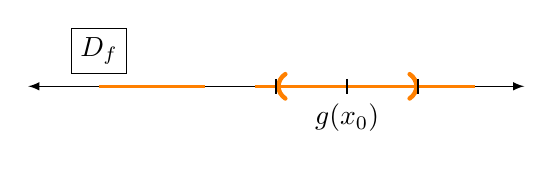
\begin{tikzpicture}[scale=0.9]
    \draw[latex-latex] (-3.5,0) -- (3.5,0) ; %edit here for the axis
    \draw[(-, ultra thick, orange] (0,0) -- (0.01,0);
    \draw[{-)}, ultra thick, orange] (2,0) -- (2.01,0);
    %\fill[opacity = 0.2, blue,rounded corners=1ex] (0,-1ex) -- (2, -1ex) -- (2, 1ex) -- (0,1ex) -- cycle;
    \draw[very thick, color=orange] (-0.3,0) -- (2.8,0);
    \draw[very thick, color=orange] (-2.5,0) -- (-1,0);
    \node[draw] at (-2.5, 0.5) {$D_f$};
    %
    \draw[shift={(0,0)}, thick, color=black] (0pt,3pt) -- (0pt,-3pt);
    \draw[shift={(0,0)}, thick, color=black] (0pt,0pt) -- (0pt,-3pt);
    %
    \draw[shift={(2,0)}, thick, color=black] (0pt,3pt) -- (0pt,-3pt);
    \draw[shift={(2,0)}, thick, color=black] (0pt,0pt) -- (0pt,-3pt);
    %
    \draw[shift={(1,0)}, thick, color=black] (0pt,3pt) -- (0pt,-3pt);
    \draw[shift={(1,0)}, thick, color=black] (0pt,0pt) -- (0pt,-3pt) node[below]
    {$g(x_0)$};
  \end{tikzpicture}
\end{figure}

So the above theorem is saying that we must have some $(g(x_0) - \e,\, g(x_0) + \e) \sub D_f$ or even that; $\displaystyle{\lim_{x\to x_0}{f(g(x))} = f(g(x_0))}$.

\begin{proof}
  Suppose $\e>0$, since $g(x_0)\in D_f^o$ and $f$ is continous at $g(x_0), \ex\d_1>0$ st, $f(t)$ is defined and
  \begin{equation}
    |f(t) - f(g(x_0))|<\e \text{ if } |t - g(x_0)| < \d_1
  \end{equation}
  Since $g$ is continuous at $x_0$, $\ex\d_2>0$ st, $g(x)$ is defined (why?) and
  \begin{equation}
    |g(x) - g(x_0)| < \d_1 \text{ if } |x - x_0|<\d_2
  \end{equation}
  Then (4) and (5) imply that,
  $$ |f(g(x)) - f(g(x_0))| < \e \text{ if } |x - x_0| < \d_2 $$

\end{proof}

\section{Boundedness}

\noindent\fbox{\parbox{0.475\textwidth}{\begin{definition}[Bounded Below]{
 A funtion $f$ is bounded below on a set $S$ if theres an $m\in\R$
 $$ f(x) \geq m \qquad\forall x\in S $$
 In this case,
 $$ V = \{ f(x) : x\in S\} $$
 has an infimum, $\a$, and we write,
 $$ \a = \inf_{x\in S}{f(x)} $$
 If $\ex x_1\in S$, such that $f(x_1) = \a$, then we say that $\a$ is the minimum of $f$ on $S$ and write:
 $$ \a = \min_{x\in S}{f(x)} $$
}\end{definition}}}\vspace{10pt}

\noindent\fbox{\parbox{0.475\textwidth}{\begin{definition}[Bounded Above]{
 $f$ is bounded above on $S$, if $\ex M\in\R$, such that, $f(x) \le M \qquad \forall x\in S$. Then we can write;
 $$ \b = \sup_{x\in S}{f(x)} $$
 If $\ex x_2\in S$, such that $f(x_2) = \b$, then we say that $\b$ is the minimum of $f$ on $S$ and write:
 $$ \b = \max_{x\in S}{f(x)} $$
}\end{definition}}}\vspace{10pt}

\noindent\fbox{\parbox{0.475\textwidth}{\begin{definition}[Bounded]{
  If $f$ is both bounded below and bounded above on a set $S$, then $f$ is bounded on $S$.
}\end{definition}}}\vspace{10pt}

\begin{theorem}[Boundedness Theorem]
  If $f$ is continuous on a finite closed interval $[a,\, b]$, then $f$ is bounded on $[a,\,b]$
\end{theorem}
\begin{tikzpicture}[declare function={f(\x)=0.3*(\x-3.5)^3-\x+7;a=1;b=6;c=4.94; t = 3;}] %starts and declares the function
 \draw[-stealth] (-0.5,0) -- (6.5,0); % draw x axis
 \draw[-stealth] (0,-0.5) -- (0,6.5); % draw y axis
 \draw[blue] plot[smooth,domain={a}:{b}] ({\x},{f(\x)}); %draws function
 \foreach \X in {a,b,t}
 {\draw[dashed] (\X,0) node[below]{$\X$} |- (0,{f(\X)}) node[left] {$f(\X)$};} %plots points and draws dashes
 % \e-neighbourhood code
 \draw[(-, ultra thick, red] (2.75,0) -- (2.76,0);
 \draw[{-)}, ultra thick, red] (3.25,0) -- (3.26,0);
 \draw[ultra thick, red] (2.75,0) -- (3.25,0);
 % \d-neighbourhood
 \draw[(-, ultra thick, red] (0, {f(3)-0.25}) -- (0, {f(3)-0.24});
 \draw[{-)}, ultra thick, red] (0, {f(3)+0.25}) -- (0, {f(3)+0.26});
 \draw[ultra thick, red] (0, {f(3)-0.25}) -- (0, {f(3)+0.25});
 %
 \node at (a,{f(a)}) [circle,fill,inner sep=1.5pt, color=blue]{};
 \node at (b,{f(b)}) [circle,fill,inner sep=1.5pt, color=blue]{};
\end{tikzpicture}
  Assume $f$ is bounded, it curves again, I promise...
\begin{proof}
  Suppose we take a $t\in[a,\,b]$. Since $f$ is continuous at $t $  $\ex $ an open interval, $t\in I_t$, st,
  \begin{equation*}
  |f(x) - f(t)|<1 \qquad\text{if $x\in I_t\cap[a,\,b]$}\tag{$*$}
\end{equation*}
  The collection $\displaystyle{\mathcal{H} = \{ I-t : a \le t \le b \}}$ is an open cover of $[a,\, b]$. Since, $[a,\, b]$ is compact, then by the Heine-Borel theorem, there exists a finite sub-cover made up of intervals $I_{t_1},\,\dots,\,I_{t_n}$. By ($*$), taking $t = t_i$, then,
  $$ |f(x) - f(t_i)|< 1 \qquad\text{if $x\in I_{t_i}\cap[a,\,b]$} $$
  Therefore,
  \begin{align*}
    |f(x)| &= |f(x) - f(t_i) + f(t_i)| \\
    &\le |f(x) - f(t_i)| + |f(t_i)| \\
    &\le 1 + |f(t_i)|\qquad \text{if $x\in I_{t_i}\cap[a,\,b]$} \tag{$**$}\\
  \end{align*}
Let $\displaystyle{M = 1 + \max_{1\le i\le n}{|f(t_i)|}}$ and since,\\ $\displaystyle{[a,\,b]\sub \bigcup_{i=1}^n{I_{t_i}\cup[a,\,b]}}$, then apply ($**$) and then
$$ |f(x)| \le M \qquad\forall x\in[a,\,b] $$
\end{proof}

\begin{theorem}[Extreme value Theorem]
  Suppose that $f$ is continuous on a finite closed interval, $[a, b]$. Let,
  $$ \a = \inf_{a\le x\le b}{f(x)}\text{ and } \b =\sup_{a\le x\le b}{f(x)} $$
  Then $\a$ and $\b$ are respectively the minimum and maximum of $f$ on $[a,\,b]$; that is there are points $x_1$ and $x_2$ in $[a,\,b]$ such that;
  $$ f(x_1) = \a \qquad f(x_2) = \b $$
\end{theorem}
\begin{proof}
  We'll show that $x_1$ exists first. Suppose for a contradiction, that there is no point $x_1 \in [a,\,b], f(x_1) = \a$. Then for $f(t) > \a\quad \forall t \in [a,\,b]$
  $$ f(t) > \frac{f(t) + \a}{2} > \a $$
  Since, $f$ is continuous at $t$, there is an open interval $I_t$ about the point $t$, st,
  $$ f(x) > \frac{f(t) + \a}{2} \qquad x\in I_t\cap[a,\, b] $$
  Then, the collection of $\displaystyle{\mathcal{H} = \{ I_t: a\le x \le b\}}$ is an open covering of $[a, \, b]$. Since $[a, \, b]$ is compact, the Heine-Borel theorem implies that there is a finite sub-covering using some open intervals $I_{t_1},\,\dots,\,I_{t_n}$ around $t_1,\,\dots,\,t_n$. Now we define:
  $$ \a_1 = \min_{1\le i \le n}{\frac{f(t_i) + \a}{2}} $$
  Then $f(t) > \a \,\forall \,t \in \bigcup_{i=1}^n{I_{t_i}\cap[a,\,b]} = [a,\,b]$, so we now have $a_1 >\a$ and hence a contradiction. So $f(x_1) = \a$ for some $x_1\in [a,\,b]$.\\

  \noindent
  To complete the proof, show that $x_2$ exists. Suppose for a contradiction, that there is no point $x_2 \in [a,\,b], f(x_2) = \b$. Then for $f(t) < \b\quad \forall t \in [a,\,b]$
  $$ f(t) < \frac{f(t) + \b}{2} < \b $$
  Since, $f$ is continuous at $t$, there is an open interval $I_t$ about the point $t$, st,
  $$ f(x) < \frac{f(t) + \b}{2} \qquad x\in I_t\cap[a,\, b] $$
  Then, the collection of $\displaystyle{\mathcal{H} = \{ I_t: a\le x \le b\}}$ is an open covering of $[a, \, b]$. Since $[a, \, b]$ is compact, the Heine-Borel theorem implies that there is a finite sub-covering using some open intervals $I_{t_1},\,\dots,\,I_{t_n}$ around $t_1,\,\dots,\,t_n$. Now we define:
  $$ \b_1 = \max_{1\le i \le n}{\frac{f(t_i) + \b}{2}} $$
  Then $f(t) < \b \,\forall \,t \in \bigcup_{i=1}^n{I_{t_i}\cap[a,\,b]} = [a,\,b]$, so we now have $\b <\b_1$ and hence a contradiction. So $f(x_2) = \b$ for some $x_2\in [a,\,b]$.
\end{proof}

\begin{theorem}[Intermediate Value Theorem]
  Suppose that $f$ is continuous on $[a,\, b]$, $f(a)\neq f(b)$, and $\mu$ is between $f(a)$ and $f(b)$. Then $f(c) = \mu$, for some $c\in [a,\, b]$
\end{theorem}
\begin{tikzpicture}[declare function={f(\x)=0.3*(\x-3.5)^3-\x+7;a=1;b=6;}] %starts and declares the function
 \draw[-stealth] (-0.5,0) -- (6.5,0); % draw x axis
 \draw[-stealth] (0,-0.5) -- (0,6.5); % draw y axis
 \draw[blue] plot[smooth,domain={a}:{b}] ({\x},{f(\x)}); %draws function
 \foreach \X in {a,b}
 {\draw[dashed] (\X,0) node[below]{$\X$} |- (0,{f(\X)}) node[left] {$f(\X)$};} %plots points and draws dashes
 \draw[dashed, thick, green] (3,0) node[below]{$c$} |- (0,{f(3)}) node[left] {$\mu$};
 \draw[dotted, thick, orange] (1, {f(1)}) -- (6, {f(6)});
 % endpoints of the graph
 \node at (a,{f(a)}) [circle,fill,inner sep=1.5pt, color=blue]{};
 \node at (b,{f(b)}) [circle,fill,inner sep=1.5pt, color=blue]{};
\end{tikzpicture}
\begin{proof}
  Suppose that $f(a) < \mu < f(b)$. The set,
  $$ S = \{ x : a \le x \le b \text{ and }f(x)\le\mu  \} $$
  is bounded and is non-empty. Let $c = \sup S$. We will show that $f(c) = \mu$. If $f(c) > \mu$, then $c > a$ and since $f$ is continuous at $c$, $\ex\e>0$,st,
  $$ f(x) > \mu \qquad\text{ if }c - \e < x \le c $$
  Therefore, $c - \e$ is an upper bound for $S$, contradicting the definition of $c$.\\
  If $f(c) < \mu$, then $c < b$ and $\ex\e>0$, st,
  $$ f(x) < \mu \text{ for } c \le x < c + \e $$
  so $c$ is not an upper bound for $S$, which again contradicts the definition of $c$. \\
  Therefore $f(c) = \mu$. The proof for $f(b) < \mu < f(a)$ is simply obtained by applying the above to the function $-f$.
\end{proof}

\subsection{Monotonics 2: God what a mess}














\end{document}
